\documentclass[10pt,twocolumn]{article}

\usepackage[margin=0.85in]{geometry}
\usepackage{amsmath,amssymb}
\usepackage{booktabs}
\usepackage{microtype}
\usepackage{xcolor}
\usepackage{tikz}
\usepackage{pgfplots}
\pgfplotsset{compat=1.16}
\usetikzlibrary{arrows.meta,positioning,shapes.geometric,backgrounds,fit,calc}
\usepackage[hidelinks]{hyperref}
\usepackage{caption}
\captionsetup{font=small,labelfont=bf}

% palette
\definecolor{pgood}{RGB}{31,119,80}
\definecolor{pbad}{RGB}{200,40,40}
\definecolor{pnode}{RGB}{38,70,120}
\definecolor{pcell}{RGB}{235,240,248}
\definecolor{pcellb}{RGB}{240,247,240}
\definecolor{pgray}{RGB}{110,110,110}

\newcommand{\code}[1]{\texttt{\small #1}}

\tikzset{
  node/.style={circle,draw=pnode,thick,fill=white,minimum size=6.5mm,
               font=\scriptsize\bfseries,inner sep=0pt},
  client/.style={rectangle,rounded corners=1pt,draw=black,thick,fill=white,
                 minimum height=7mm,minimum width=11mm,font=\scriptsize\bfseries},
  db/.style={cylinder,shape border rotate=90,draw=pnode,fill=pcell,
             aspect=0.35,minimum height=9mm,minimum width=9mm,
             font=\tiny,align=center,inner sep=1pt},
  good/.style={-{Stealth[length=2mm]},pgood,thick},
  goodr/.style={-{Stealth[length=2mm]},pgood,thick,dashed},
  bad/.style={-{Stealth[length=2mm]},pbad,thick,dash pattern=on 1pt off 1.4pt},
  meshgood/.style={pgood,thick},
  meshbad/.style={pbad,thick,dash pattern=on 1pt off 1.4pt},
}

\title{\vspace{-3.5em}\bfseries pillar-UDP: Clustered Multipath Congestion
Avoidance and Redundant Delivery over Lossy Networks}
\author{\normalsize pillar engineering \quad(machine-checked design note)}
\date{\normalsize 2026-08-31}

\begin{document}
\maketitle

\begin{abstract}
\noindent
TCP and QUIC treat packet loss as the signal to \emph{slow down}: a single
path, a congestion window, additive-increase/multiplicative-decrease backoff.
On a link where loss is the link's own fault---radio, satellite, jamming,
cell-tower handoff---that reflex collapses throughput to near zero. pillar-UDP
takes the opposite posture. Its unit of congestion control is not a window on
one path but \emph{the whole cell}: a message is delivered by spraying a
\emph{bounded} number of redundant, content-addressed datagrams across a
topologically dispersed set of nodes and letting the receiver deduplicate by
CID. Loss and latency are absorbed by redundancy; congestion is avoided by
\emph{finding a good route}, not by throttling. We give two TLA\textsuperscript{+}
models---a one-to-many non-node client and a many-to-many inter-cell full
mesh---each with multiple nodes and multiple links, at least one adversarially
lossy, and machine-check with TLC that (i)~delivery always \emph{routes around}
the lossy links whenever the cell stays reachable by any dispersed path
(liveness), (ii)~redundant copies arriving at multiple nodes are accepted
exactly once (CID dedup, safety), and (iii)~per-round fan-out never exceeds the
configured redundancy allowance (safety). We contrast this with the
single-client, single-path congestion posture of TCP and QUIC. The redundancy
header format and the quantitative scaling of the loss/bandwidth trade are the
subject of a companion paper.
\end{abstract}

\section{The problem: loss is not always congestion}
The two guarantees of TCP---reliable, ordered byte delivery---are enforced by
windows that regulate in-flight data, and those windows are a feedback loop
tuned by observed loss. The design assumes loss \emph{means} congestion, so the
polite response is to back off. On a marginal link the assumption is simply
false: loss there is the medium degrading, and backing off makes a recoverable
link useless. The empirical cliff is steep---on a $20\,\mathrm{ms}$ path the
first $1\%$ of loss already removes about $80\%$ of TCP throughput, and past
roughly $17\%$ loss TCP ceases to function at all; higher round-trip time makes
recovery from each loss event dramatically slower~\cite{grayson}. QUIC modernises
loss recovery and removes head-of-line blocking across streams, but its
congestion posture is the same family: one path, one connection, a
loss-driven congestion controller that throttles under loss.

pillar's deployments are exactly where this bites: cells span multiple sites on
distinct provider prefixes, clients reach the cell over the open internet or
worse, and inter-cell links cross congested or adversarial transit. pillar-UDP
is the protocol for that regime.

\section{Posture: redundancy plus clustered multipath routing}
pillar-UDP's design posture is twofold, and each half maps onto any protocol
that supports a subset of its features:
\begin{enumerate}\itemsep2pt
  \item \textbf{Variable loss/latency tolerance through redundancy.} A message
  is a small, PGP-signed, content-addressed (CID) unit. The sender emits
  redundant copies; the receiver deduplicates by CID, so at-least-once
  transport plus CID identity yields exactly-once \emph{processing}. Fan-out per
  round is capped by a \emph{redundancy allowance} carried in the header, so a
  known-bad link states its characteristics up front.
  \item \textbf{Automatic, dynamic, clustered multipath congestion avoidance.}
  The control variable is \emph{route and source selection}, not window size.
  Redundant datagrams are emitted from as dispersed a set of node addresses as
  possible---steered by topology tier, GeoIP, and measured latency/loss---to
  maximise the chance that some path around the bad link is good.
\end{enumerate}
Because trust is carried by the signature on each message and not by its origin
address, the node that \emph{replies} need not be the node that
\emph{ingested}: a cell can answer from whichever dispersed nodes have the best
paths to the client. How many nodes can actually reply depends on the client's
address family---end-to-end IPv6 addressing makes the dispersed reply mesh
native, while IPv4 behind NAT constrains it (\S\ref{sec:replypath}).

\begin{figure}[t]
\centering
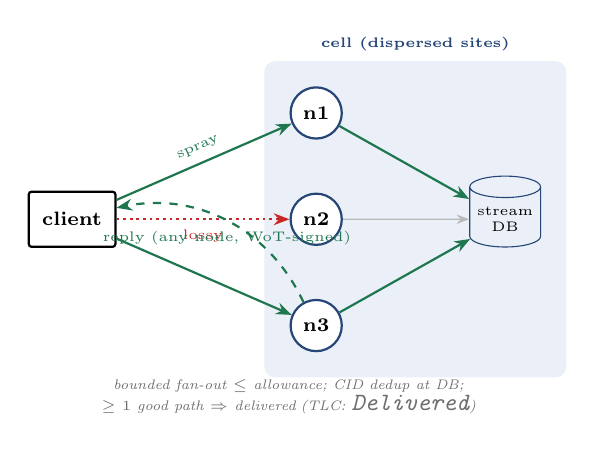
\begin{tikzpicture}[node distance=6mm]
  \node[client] (c) at (0,0) {client};
  % dispersed ingest nodes
  \node[node] (n1) at (3.1, 1.35) {n1};
  \node[node] (n2) at (3.1, 0.0)  {n2};
  \node[node] (n3) at (3.1,-1.35) {n3};
  \node[db]   (db) at (5.5, 0.0) {stream\\DB};
  % cell backdrop
  \begin{scope}[on background layer]
    \node[fill=pcell,rounded corners,fit=(n1)(n2)(n3)(db),
          inner sep=3.2mm,label={[font=\tiny\bfseries,pnode]above:cell (dispersed sites)}] {};
  \end{scope}
  % spray: two good, one lossy
  \draw[good]  (c) -- node[above,font=\tiny,pgood,sloped]{spray} (n1);
  \draw[bad]   (c) -- node[below,font=\tiny,pbad,sloped]{lossy} (n2);
  \draw[good]  (c) -- (n3);
  % dedup into DB
  \draw[good]  (n1) -- (db);
  \draw[good]  (n3) -- (db);
  \draw[gray!55,-{Stealth[length=1.6mm]}] (n2) -- (db);
  % reply from a different node than ingest
  \draw[goodr] (n3) to[bend right=38] node[below,font=\tiny,pgood]{reply (any node, WoT-signed)} (c);
  \node[font=\tiny\itshape,pgray,align=center] at (2.75,-2.25)
     {bounded fan-out $\le$ allowance; CID dedup at DB;\\
      $\ge 1$ good path $\Rightarrow$ delivered\;(TLC: \code{Delivered})};
\end{tikzpicture}
\caption{\textbf{One-to-many (ingress class 2).} A non-node client sprays
redundant datagrams to a dispersed set of ingest nodes. The path to \code{n2}
is lossy; copies still reach \code{n1} and \code{n3}, the streaming DB
deduplicates by CID, and the reply returns from a \emph{different} node than
ingested it. Modeled in \code{PillarUdpClient.tla}.}
\label{fig:onetomany}
\end{figure}

\section{Formal models and what TLC proves}
We model pillar-UDP at the level at which its guarantees live---delivery,
deduplication, and bounded redundancy under an adversarial lossy channel---in
two TLA\textsuperscript{+} specifications, following the lossy-channel plus
strong-fairness idiom pillar already uses for anti-entropy replication. Both
make the pending work \emph{monotone} so that an adversary cannot destroy
in-flight progress, and both encode the route-around premise as a standing
constraint on the adversary: it may flip \emph{any} links lossy at any time,
\emph{provided the cell stays reachable by at least one dispersed path}. The
theorem in each case is that pillar-UDP always finds that path, with no window
control.

\paragraph{One-to-many (\code{PillarUdpClient}).}
A client sprays subsets of dispersed nodes (each spray bounded by the
allowance; coverage accumulates monotonically across retransmit rounds). A copy
reaches any node whose path is currently good; the first copy anywhere injects
the message, later copies dedup. TLC checks:
\begin{itemize}\itemsep1pt
  \item \textbf{\code{ExactlyOnce}} (safety): the message is injected at most
  once, though \code{received} may grow to several nodes.
  \item \textbf{\code{SprayWidthBounded}} (safety): no round exceeds the
  allowance.
  \item \textbf{\code{Delivered}} (liveness, $\Diamond$): the message is
  eventually injected despite arbitrarily many loss bursts.
\end{itemize}

\paragraph{Many-to-many (\code{PillarUdpMesh}).}
Two cells, each at several sites, form a full mesh of site-to-site links; a
flow of messages is spread across the mesh. Any link may be lossy; delivery of
each message counts once (CID dedup) regardless of how many sites redundantly
forward it. TLC checks \textbf{\code{ExactlyOnce}} (safety) and
\textbf{\code{MeshCompletes}} (liveness, $\Diamond$): the entire flow completes
by routing around lossy links over the surviving site pairs.

\begin{table}[t]
\centering
\small
\begin{tabular}{@{}lrrl@{}}
\toprule
model & distinct states & depth & result \\
\midrule
\code{PillarUdpClient} & 329   & 7  & no error \\
\code{PillarUdpMesh}   & 3\,840 & 10 & no error \\
\bottomrule
\end{tabular}
\caption{TLC exhaustive model-checking results (deadlock checking on). Every
listed invariant and liveness property holds over the complete state space of
each finite instance. Both specs run in pillar's \code{specs/check.sh} gate.}
\label{tab:tlc}
\end{table}

Table~\ref{tab:tlc} reports the actual TLC output. These are \emph{logical}
guarantees---exactly-once delivery and route-around progress hold over every
interleaving of spraying, delivery, and adversarial loss. They are not
throughput measurements; the quantitative loss/bandwidth trade is analytic
(\S\ref{sec:redundancy}) and is treated fully in the companion paper.

\begin{figure}[t]
\centering
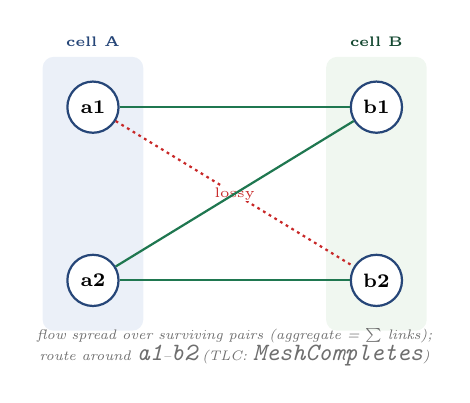
\begin{tikzpicture}
  % Cell A sites
  \node[node] (a1) at (0, 1.1) {a1};
  \node[node] (a2) at (0,-1.1) {a2};
  % Cell B sites
  \node[node] (b1) at (3.6, 1.1) {b1};
  \node[node] (b2) at (3.6,-1.1) {b2};
  \begin{scope}[on background layer]
    \node[fill=pcell,rounded corners,fit=(a1)(a2),inner sep=3mm,
          label={[font=\tiny\bfseries,pnode]above:cell A}] {};
    \node[fill=pcellb,rounded corners,fit=(b1)(b2),inner sep=3mm,
          label={[font=\tiny\bfseries,pgood!60!black]above:cell B}] {};
  \end{scope}
  % full mesh 2x2
  \draw[meshgood] (a1) -- (b1);
  \draw[meshbad]  (a1) -- node[pos=0.5,font=\tiny,pbad,fill=white,inner sep=0.5pt]{lossy} (b2);
  \draw[meshgood] (a2) -- (b1);
  \draw[meshgood] (a2) -- (b2);
  \node[font=\tiny\itshape,pgray,align=center] at (1.8,-1.95)
     {flow spread over surviving pairs (aggregate = $\sum$ links);\\
      route around \code{a1}--\code{b2}\;(TLC: \code{MeshCompletes})};
\end{tikzpicture}
\caption{\textbf{Many-to-many (ingress class 3).} Two cells present at multiple
sites form a full mesh. The \code{a1}--\code{b2} link is lossy; the A$\to$B flow
completes over the other three pairs, aggregating their bandwidth instead of
bottlenecking on one connection. Modeled in \code{PillarUdpMesh.tla}.}
\label{fig:manytomany}
\end{figure}

\section{Automatic geographic load balancing}
Neither model contains a load balancer, a scheduler, or a route table. Delivery
happens over \emph{whatever dispersed path is currently good}; that is the load
balancing. Because pillar-ipam binds addresses to topology labels (region,
rack, node) and sites hold distinct prefixes, ``spray from a dispersed set of
IPs'' is a topology-diversity query: diverse tiers give diverse prefixes give
diverse paths. A node processes a message it can serve locally and forwards it
under load; work therefore migrates to where capacity and good paths are, with
near-zero configuration. The safety obligation that keeps this sound---that only
idempotent messages may be processed opportunistically, while exclusive effects
route to the coordination-core lease holder---is orthogonal to the transport and
is modeled elsewhere; here every message is idempotent (CID dedup), so
\code{ExactlyOnce} is exactly the property that opportunistic, redundant,
multi-node delivery must not violate, and TLC confirms it does not.

\section{Reply-path addressing: IPv6 versus IPv4/NAT}\label{sec:replypath}
The dispersed-reply property of \S2---any well-placed node may answer, not only
the one that ingested---requires that those nodes can actually \emph{reach} the
client, and how many can is decided entirely by the client's address family. The
connection itself is always client-initiated: on joining a cell the client
receives the cell's node list and opens redundant connections to several
reachable ingest nodes (a deployment is expected to keep some nodes' pillar-UDP
port publicly reachable). Because the client dials outbound, each connection
opens its own return path through any intervening NAT, so the \emph{base} case
needs no hole punching, and a degrading connection is simply abandoned for the
remaining ones. Reply-node \emph{diversity}---how many distinct nodes can send
\emph{back} to the client---then splits into three tiers:
\begin{itemize}\itemsep2pt
  \item \textbf{IPv6 (GUA)---preferred, scales.} With a global address on the
  client, any cell node sends to it directly with \emph{no} per-peer NAT state.
  Reply-node diversity spans the full redundancy fan-out, so this is the only
  tier in which the clustered congestion-avoidance advantage of \S2 is realised
  end to end for a client, not just for the inter-cell mesh of
  Fig.~\ref{fig:manytomany}.
  \item \textbf{IPv4 $+$ DCUtR---partial.} Behind NAT, the publicly reachable
  ingest node coordinates DCUtR (direct-connection-upgrade-through-relay) hole
  punches so that \emph{additional} nodes obtain direct paths to the client,
  widening diversity past the single ingest. But each punched peer consumes a
  distinct port mapping on the client's NAT: DCUtR removes the single-node
  bottleneck only to replace it with a \emph{port-exhaustion} one, so this tier
  cannot scale to a large fan-out.
  \item \textbf{IPv4, no DCUtR---floor.} Only the port-forwarded ingest node(s)
  the client actually dialed can answer, over the client-initiated mappings.
  Delivery is effectively single-path---the regime pillar-UDP's redundancy is
  least able to improve.
\end{itemize}
IPv6 is therefore strictly preferred, for a structural reason rather than a
performance heuristic: DCUtR trades one bottleneck for another, whereas a global
address removes the bottleneck outright. The IPv6-native reply mesh is what lets
a single client---not only an inter-cell mesh---enjoy the full dispersed-path
redundancy the models prove.

\section{Redundancy characteristics}\label{sec:redundancy}
Redundancy is what buys loss tolerance. If a message rides in $W$ consecutive or
parallel copies over paths with independent loss probability $p$, it is lost
only if all $W$ copies drop:
\[
  P(\text{undelivered}) = p^{\,W}.
\]
Crucially, pillar-UDP's dispersion makes the independence assumption
\emph{hold}: copies sent from geographically and AS-diverse nodes do not share a
bursty bottleneck, unlike $W$ copies on one link. Figure~\ref{fig:reliability}
plots $p^{W}$: at $30\%$ loss, $W{=}10$ already drives residual loss below
$10^{-5}$, and $W{=}20$ below $10^{-10}$. The cost is bandwidth---fan-out scales
with $W$---which is why the allowance is a per-connection budget and why the
detailed loss/bandwidth scaling and header encoding are a separate paper. The
model here proves the \emph{qualitative} guarantee that redundancy plus a good
path always completes; the figure shows the \emph{rate} at which redundancy buys
reliability.

\begin{figure}[t]
\centering
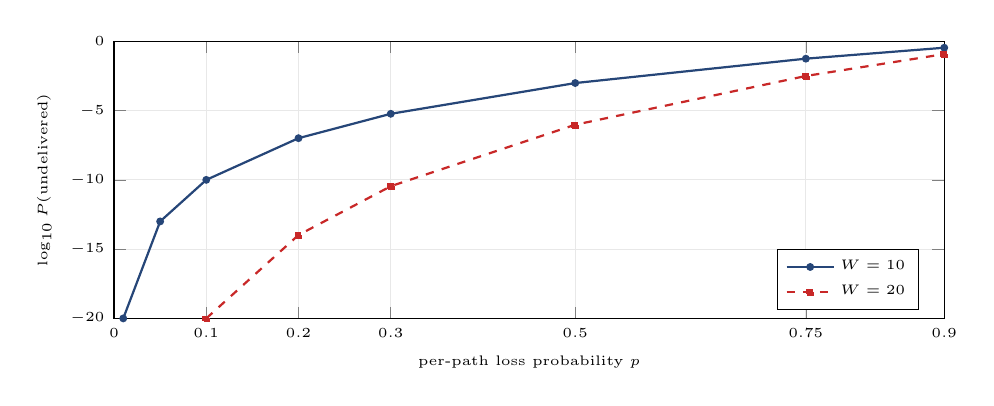
\begin{tikzpicture}
\begin{axis}[
  width=\columnwidth, height=5.1cm,
  xlabel={per-path loss probability $p$},
  ylabel={$\log_{10} P(\text{undelivered})$},
  xmin=0,xmax=0.9, ymin=-20, ymax=0,
  xtick={0,0.1,0.2,0.3,0.5,0.75,0.9},
  ytick={0,-5,-10,-15,-20},
  legend pos=south east, legend style={font=\tiny},
  tick label style={font=\tiny}, label style={font=\tiny},
  grid=both, grid style={gray!18},
]
% log10(p^W) points, from the redundancy math
\addplot[pnode,thick,mark=*,mark size=1pt] coordinates {
  (0.01,-20)(0.05,-13.0)(0.10,-10.0)(0.20,-6.99)(0.30,-5.23)(0.50,-3.01)(0.75,-1.25)(0.90,-0.46)};
\addlegendentry{$W=10$}
\addplot[pbad,thick,mark=square*,mark size=1pt,dashed] coordinates {
  (0.10,-20)(0.20,-13.98)(0.30,-10.46)(0.50,-6.02)(0.75,-2.50)(0.90,-0.92)};
\addlegendentry{$W=20$}
\end{axis}
\end{tikzpicture}
\caption{Residual loss $p^{W}$ vs.\ per-path loss for redundancy windows
$W{=}10$ and $W{=}20$ (points from the $p^{W}$ table; dispersed paths make the
independence assumption realistic). Lower is better; note the log scale.}
\label{fig:reliability}
\end{figure}

\section{Contrast with TCP and QUIC}
Table~\ref{tab:contrast} summarises the posture difference. The essential point
is architectural, not parametric: TCP and QUIC place congestion control on a
single client over a single path and react to loss by \emph{reducing} the
offered rate; pillar-UDP places it on a cluster over many paths and reacts to
loss by \emph{relocating} the offered traffic. On a healthy link QUIC is the
right tool and remains pillar's default; pillar-UDP is selected---as an
additional libp2p transport---only where the link itself is the problem, the
regime in which single-path congestion control degrades toward zero.

\begin{table}[t]
\centering\small
\begin{tabular}{@{}p{0.30\columnwidth}p{0.30\columnwidth}p{0.30\columnwidth}@{}}
\toprule
 & TCP / QUIC & pillar-UDP \\
\midrule
unit of control & one connection, one path & the cell: many nodes, many paths \\
loss reaction & shrink congestion window & re-route / re-disperse redundancy \\
reliability via & retransmit after RTT & redundant copies ($p^{W}$) + NACK \\
identity / trust & 5-tuple / TLS cert & per-message WoT signature (CID) \\
reply source & same connection & any dispersed node \\
lossy-link limit & collapses past $\sim$17\% loss \cite{grayson} & delivers while $\ge 1$ path is good \\
\bottomrule
\end{tabular}
\caption{Congestion-handling posture. QUIC improves loss recovery and stream
multiplexing over TCP but keeps the single-path, window-throttled posture.}
\label{tab:contrast}
\end{table}

\section{Scope and limitations}
The models are finite instances (three ingest nodes; a $2{\times}2$ mesh); they
establish the protocol's logical guarantees, not a performance bound. The
redundancy posture is deliberately \emph{not} congestion-controlled in the TCP
sense: it trades bandwidth for reliability and must therefore be gated to
degraded/adversarial links and bounded by the allowance, never run as an
open-internet default. Bulk transfer is a distinct problem addressed by
erasure-coded, CID-verified chunking over the same dispersed spray, and the
redundancy-header format and its loss/bandwidth scaling are the subject of the
companion paper. The anti-amplification obligation (return-routability before
committing redundant replies) and the idempotent-vs-exclusive processing
classification are specified in their own models.

\section{Conclusion}
pillar-UDP replaces ``find the right window'' with ``find the right route, and
spray enough copies to survive the ones that fail.'' Two machine-checked
TLA\textsuperscript{+} models show that this delivers exactly once and always
routes around lossy links as long as the cell stays reachable by any dispersed
path---for a non-node client (one-to-many) and for an inter-cell full mesh
(many-to-many) alike. The result is automatic geographic load balancing and
aggregate-bandwidth cell-to-cell transport with near-zero configuration, in
precisely the lossy, high-latency regime where single-path congestion control
fails.

\begin{thebibliography}{9}
\small
\bibitem{grayson} G.~Head, \emph{Reliable Delivery Over Horrible Networks},
2026. \url{https://blog.graysonhead.net/posts/reliable-delivery/}
\bibitem{tribes} M.~Frohnmayer and T.~Gift, \emph{The TRIBES Engine Networking
Model}, 2000.
\bibitem{tlaplus} L.~Lamport, \emph{Specifying Systems}, Addison-Wesley, 2002.
\end{thebibliography}

\end{document}
